\documentclass{standalone}
\usepackage{tikz}
\usepackage{pgfplots}
\pgfplotsset{width=32cm,height=18cm,compat=1.3}
\pgfplotsset{every tick label/.append style={font=\Huge}}
\usepackage{filecontents}

\usetikzlibrary{patterns}

\definecolor{citrine}{rgb}{0.89, 0.82, 0.04}

\begin{document}
	\centering
		\vspace{1.5em}
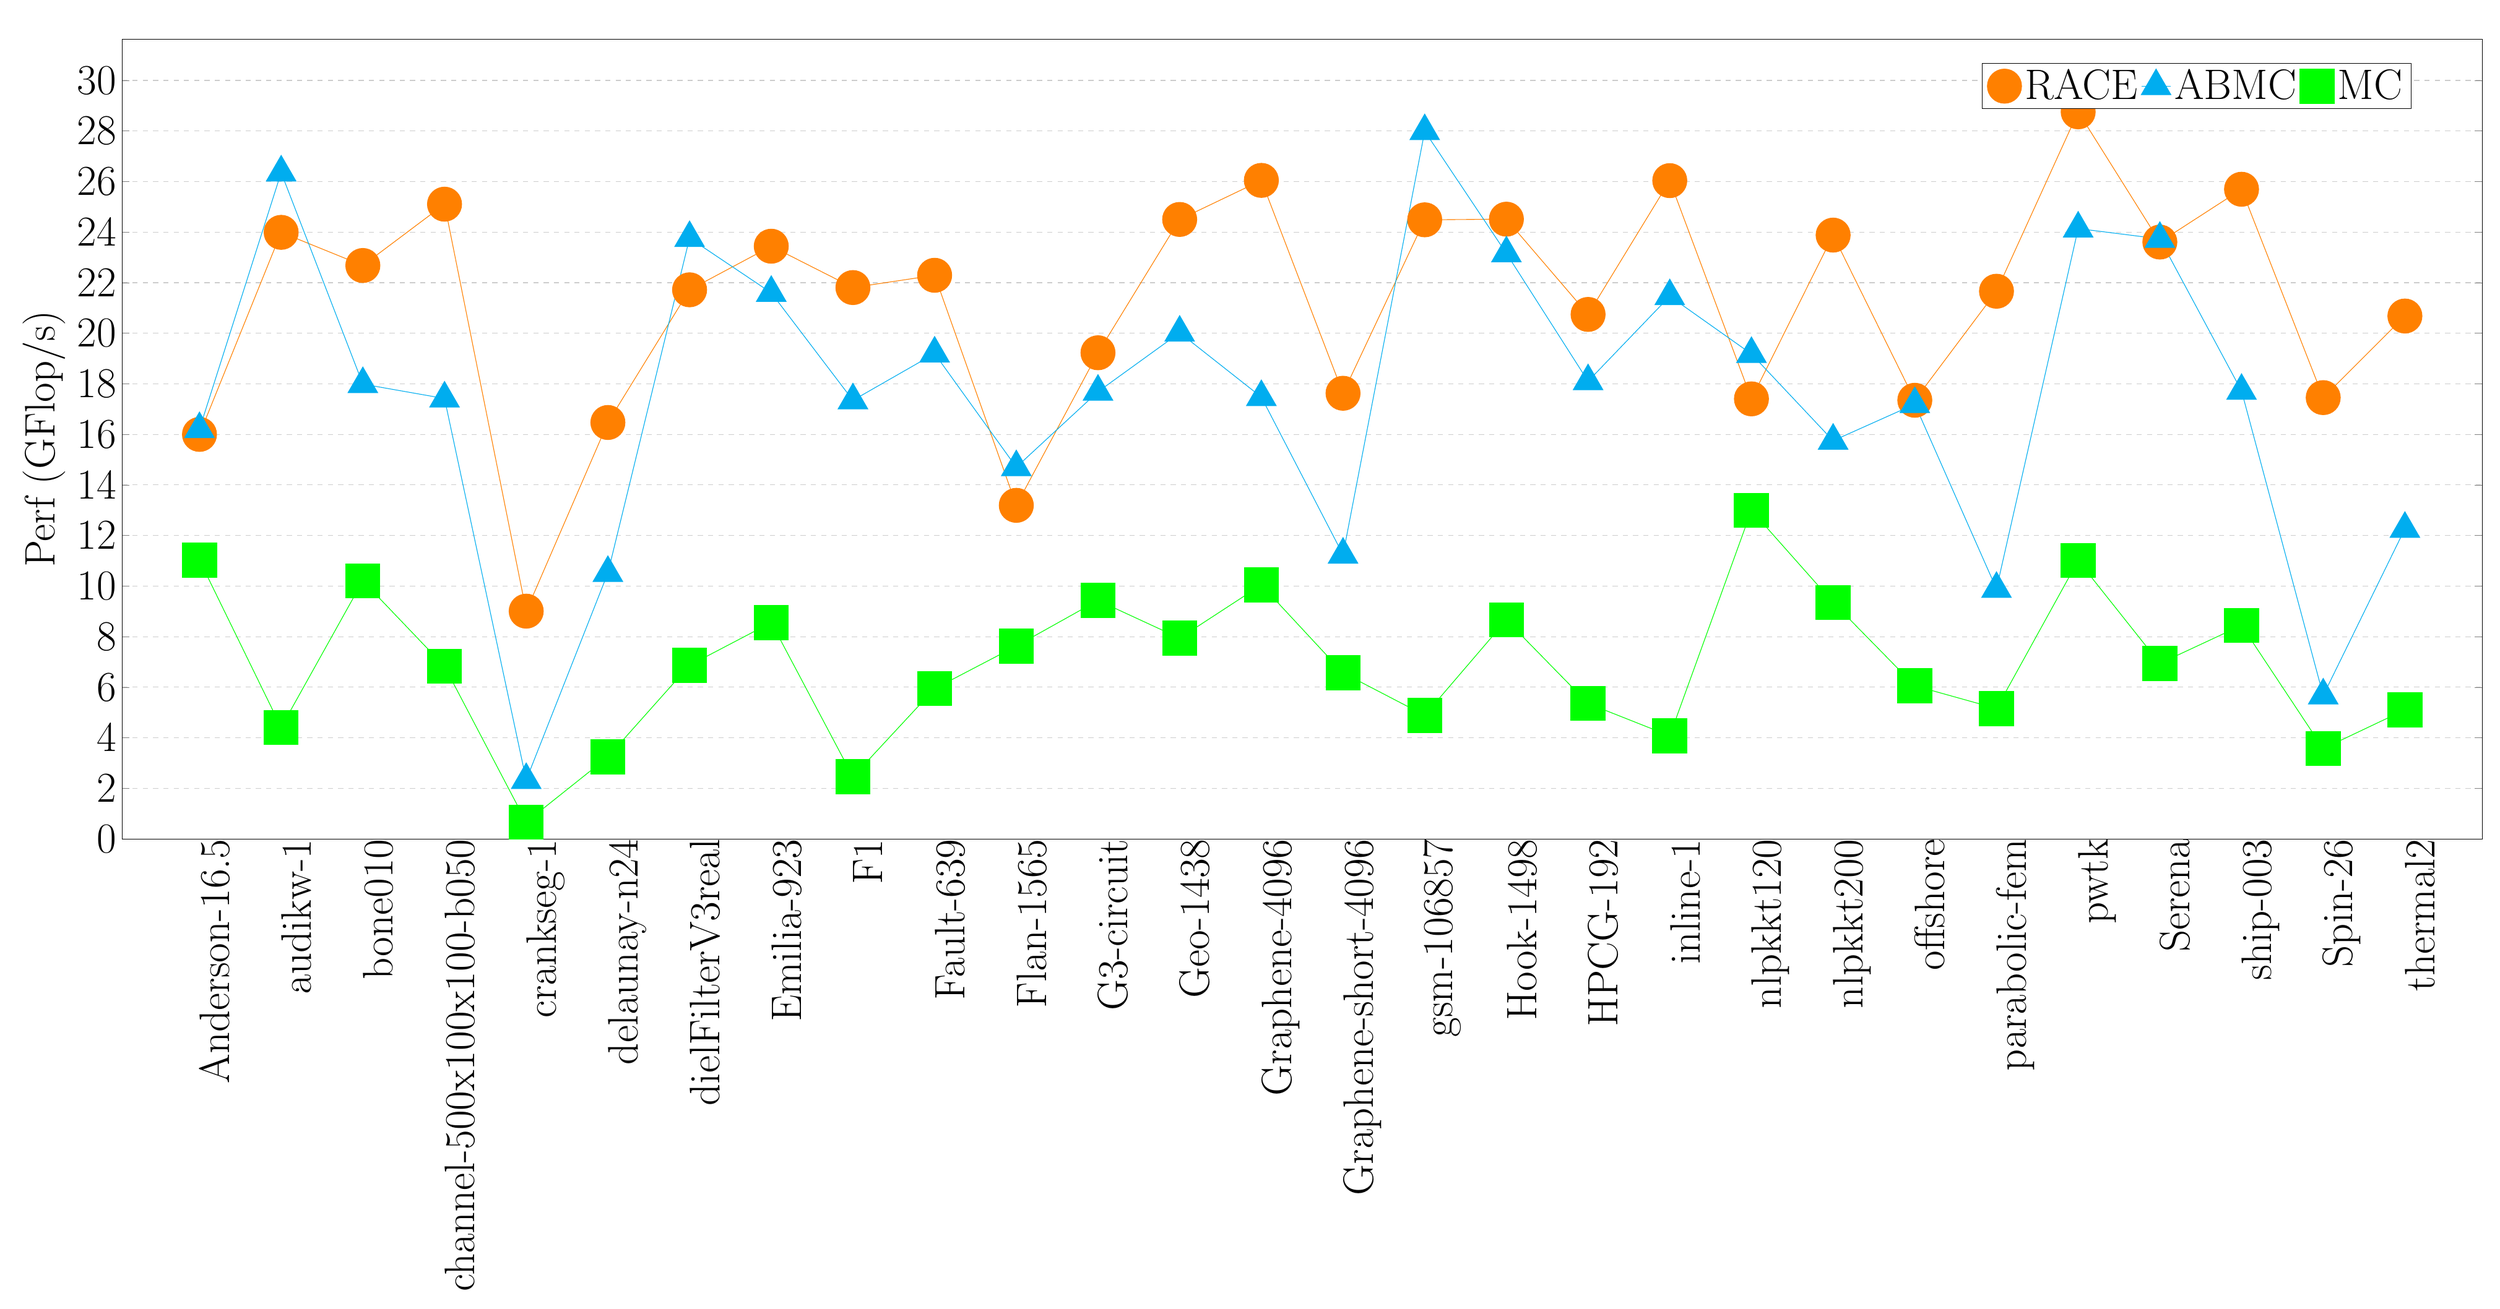
\begin{tikzpicture}
		%	\node at (13.25,15) {\LARGE{}};
			\begin{axis}[
		%	xmin=0.25, xmax=7.25,
			ymin=0, %ymax=3.25,
			xtick={1, 2, 3, 4, 5, 6, 7, 8, 9, 10, 11, 12, 13, 14, 15, 16, 17, 18, 19, 20, 21, 22, 23, 24, 25, 26, 27, 28},
		%	ytick={0,0.5,1,1.5,2,2.5,3},
			xticklabels={Anderson-16.5, audikw-1, bone010, channel-500x100x100-b050, crankseg-1, delaunay-n24, dielFilterV3real, Emilia-923, F1, Fault-639, Flan-1565, G3-circuit, Geo-1438, Graphene-4096, Graphene-short-4096, gsm-106857, Hook-1498, HPCG-192, inline-1, nlpkkt120, nlpkkt200, offshore, parabolic-fem, pwtk, Serena, ship-003, Spin-26, thermal2},
			width  = 50cm,
			height = 18cm,
			major x tick style = transparent,
			%	minor ytick={1, 5, 10, 15, 20, 25, 30 ,35,40},
			grid = minor,	
			%add_bar_commands
			ymajorgrids = true,
			grid style={dashed, gray!40},
			ylabel = {\Huge{Perf (GFlop/s)}},
		%	symbolic x coords={Graphene-2048-2048, Graphene-4096-4096, Spin-24-24-24},
			x tick label style={rotate=90, anchor=north east, inner sep=0mm, font={\Huge}},
			tick label style={font={\Huge}},
			scaled y ticks = false,
			enlarge x limits=0.035,
			legend cell align=left,
			legend style={font=\Huge},
			legend columns=-1,
			legend style={
				%at={(1,1.05)},
				%anchor=south east,
				%column sep=1ex,
				legend pos=north east
			},
			%spl_legend_code
			title= {\Huge\scalebox{1.5}{{}}}
			]

\addplot[mark=*, mark size=10pt, mark options={orange}, draw=orange , y filter/.code={\pgfmathparse{\pgfmathresult*1000}\pgfmathresult}] plot coordinates{(1,.01599864878048780487) (2,.02399082156862745098) (3,.02267958952380952380) (4,.02510504077669902912) (5,.00900787058823529411) (6,.01646992815533980582) (7,.02171823235294117647) (8,.02344252212389380530) (9,.02180695392156862745) (10,.02229240775862068965) (11,.01319281297297297297) (12,.01922798000000000000) (13,.02450105000000000000) (14,.02604580198019801980) (15,.01762574356435643564) (16,.02448616138613861386) (17,.02451201346153846153) (18,.02074416666666666666) (19,.02603642900000000000) (20,.01740427678571428571) (21,.02388196213592233009) (22,.01734887572815533980) (23,.02166124666666666666) (24,.02875698349514563106) (25,.02360650306122448979) (26,.02569509902912621359) (27,.01745434205607476635) (28,.02068126336633663366)};
\addplot[mark=triangle*, mark size=10pt, mark options={cyan}, draw=cyan , y filter/.code={\pgfmathparse{\pgfmathresult*1000}\pgfmathresult}] plot coordinates{(1,.01620802685185185185) (2,.02635741263157894736) (3,.01798808102189781021) (4,.01741837433628318584) (5,.00232788800000000000) (6,.01051870396825396825) (7,.02376578269230769230) (8,.02159829747899159663) (9,.01734675689655172413) (10,.01919496793893129770) (11,.01470168786127167630) (12,.01768691758241758241) (13,.02002128257575757575) (14,.01747477478260869565) (15,.01124004000000000000) (16,.02799141428571428571) (17,.02315846929824561403) (18,.01810203070175438596) (19,.02146467090909090909) (20,.01917990089285714285) (21,.01574933947368421052) (22,.01719446067415730337) (23,.00988710797872340425) (24,.02413927735849056603) (25,.02373265049504950495) (26,.01772064761904761904) (27,.00567272894736842105) (28,.01226363422818791946)};
\addplot[mark=square*, mark size=10pt, mark options={green}, draw=green , y filter/.code={\pgfmathparse{\pgfmathresult*1000}\pgfmathresult}] plot coordinates{(1,.01102522900763358778) (2,.00441205042016806722) (3,.01020725035971223021) (4,.00682350500000000000) (5,.00066384433333333333) (6,.00324062602739726027) (7,.00686638611111111111) (8,.00855649387755102040) (9,.00245966940298507462) (10,.00594174901960784313) (11,.00762774873096446700) (12,.00943212622950819672) (13,.00793950000000000000) (14,.01004545196850393700) (15,.00656809356725146198) (16,.00488760853658536585) (17,.00865904402985074626) (18,.00535589926470588235) (19,.00407591259259259259) (20,.01299564552845528455) (21,.00935312741935483870) (22,.00605653706896551724) (23,.00515510862944162436) (24,.01100738833333333333) (25,.00694022605042016806) (26,.00844510776699029126) (27,.00356967286821705426) (28,.00510320066225165562)};
	%addplot cmd

	\legend{RACE, ABMC, MC}

	\end{axis}			
\end{tikzpicture}

\end{document}

